\documentclass{report}
\usepackage{hyperref}
\usepackage{graphicx}
\usepackage{wrapfig}
\graphicspath{ {./th_images/} }
\title{}
\date{}

\begin{document}
 
  \pagenumbering{gobble}
  \maketitle
  \newpage
  \pagenumbering{arabic}
  \setlength{\parskip}{2em}

\begin{titlepage}
   \begin{center}
	   \LARGE
       \textbf{UNIVERSITATEA “ALEXANDRU IOAN CUZA” DIN IAȘI}\\
 	   \textbf{FACULTATEA DE INFORMATICĂ}\\

       \vspace{1cm}
       
\includegraphics[width=0.4\textwidth]{fii}
 
       \vspace{1.5cm}
 	   \textbf{LUCRARE DE LICENȚĂ}\\

       \textbf{TimelineGenerator}\\
	   propusă de
 	   \textbf{Oana-Maria Hriscu}
       \vfill 
       \vspace{0.8cm}
 
 
       \textbf{Sesiunea}: Iulie, 2019\\
       \textbf{Coordonator științific:} Prof.Dr. Cristea Dan
      
 
   \end{center}
\end{titlepage}
\begin{titlepage}
   \begin{center}
	   \Large
       \textbf{UNIVERSITATEA “ALEXANDRU IOAN CUZA” DIN IAȘI}\\
 	   \textbf{FACULTATEA DE INFORMATICĂ}\\


       \vspace{3cm}
	   \Huge
       \textbf{TimelineGenerator}\\

	 \vspace{1cm}
	   \normalsize
 	   \textbf{Oana-Maria Hriscu}
       \vfill 
       \vspace{0.8cm}
 
 \Large
       \textbf{Sesiunea}: Iulie, 2019\\
       \textbf{Coordonator științific:} Prof.Dr. Cristea Dan
      
 
   \end{center}
\end{titlepage}
\centerline{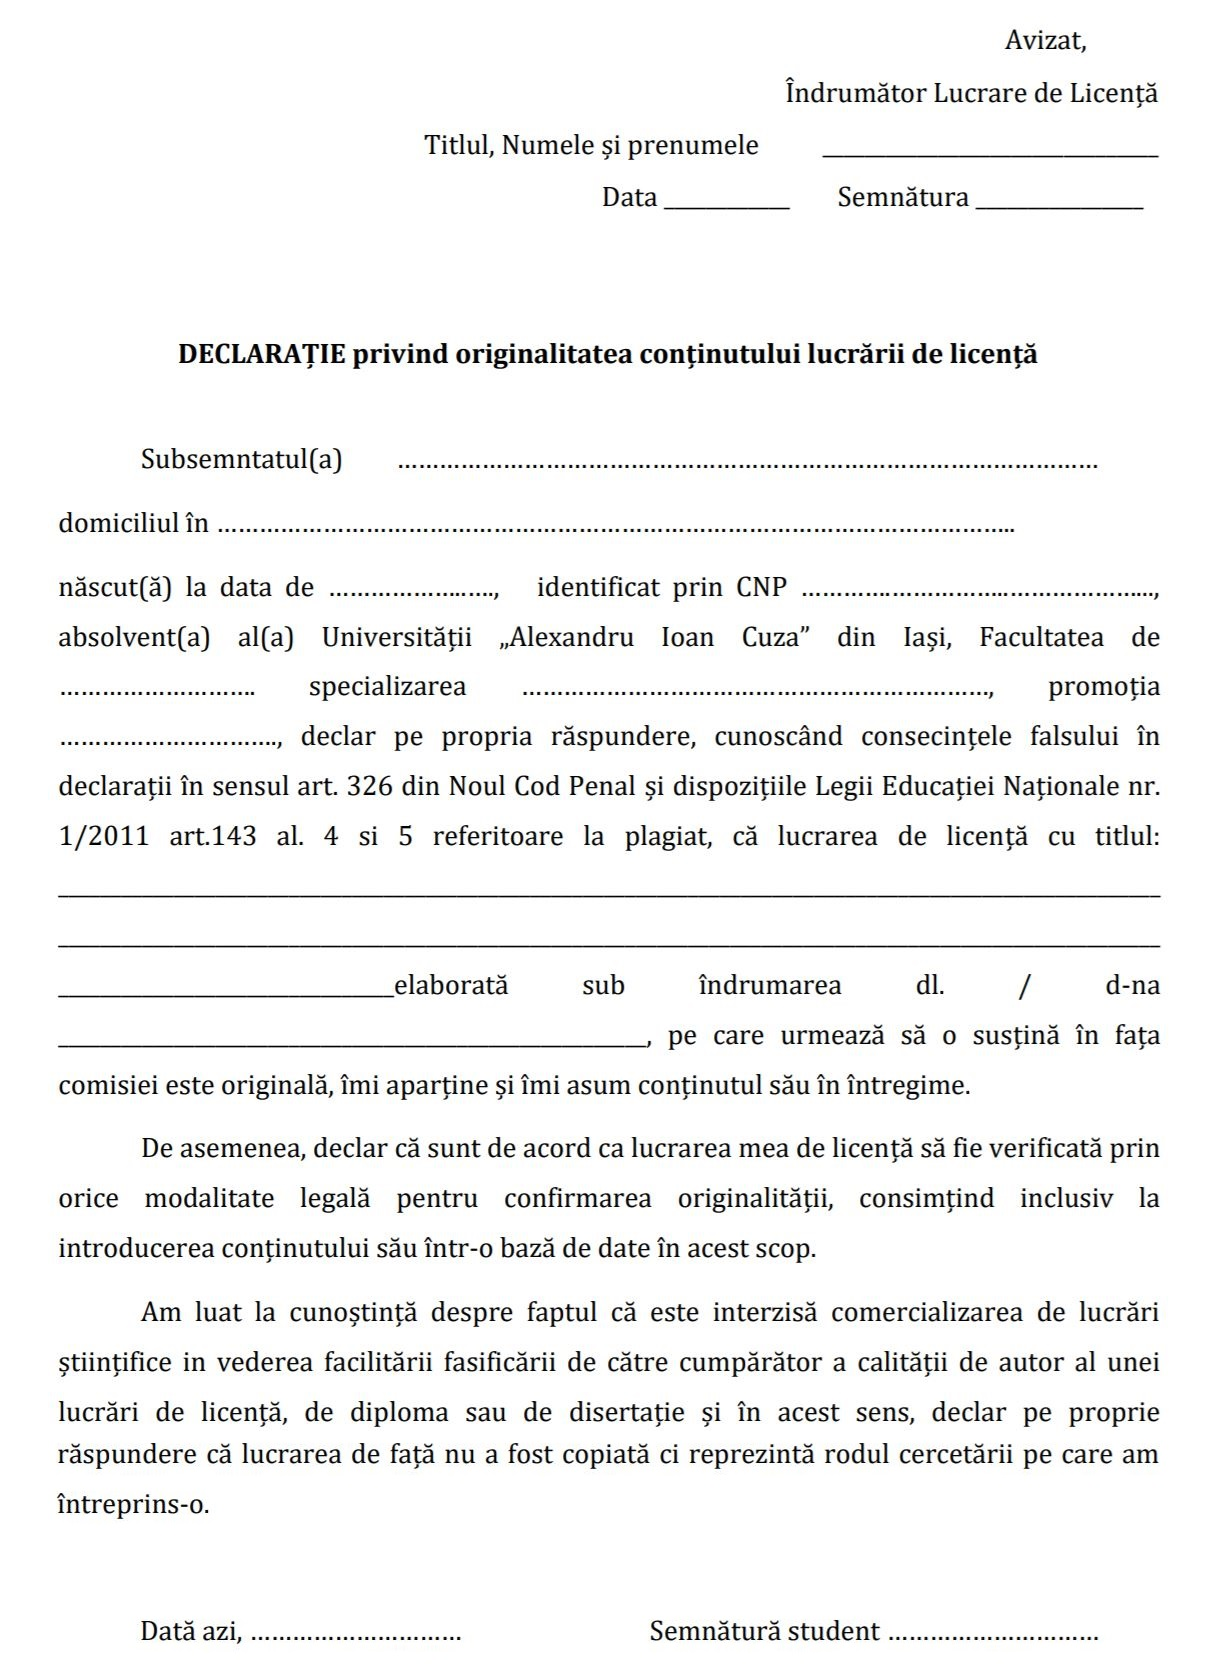
\includegraphics[scale=1.1]{anexa4}}
\centerline{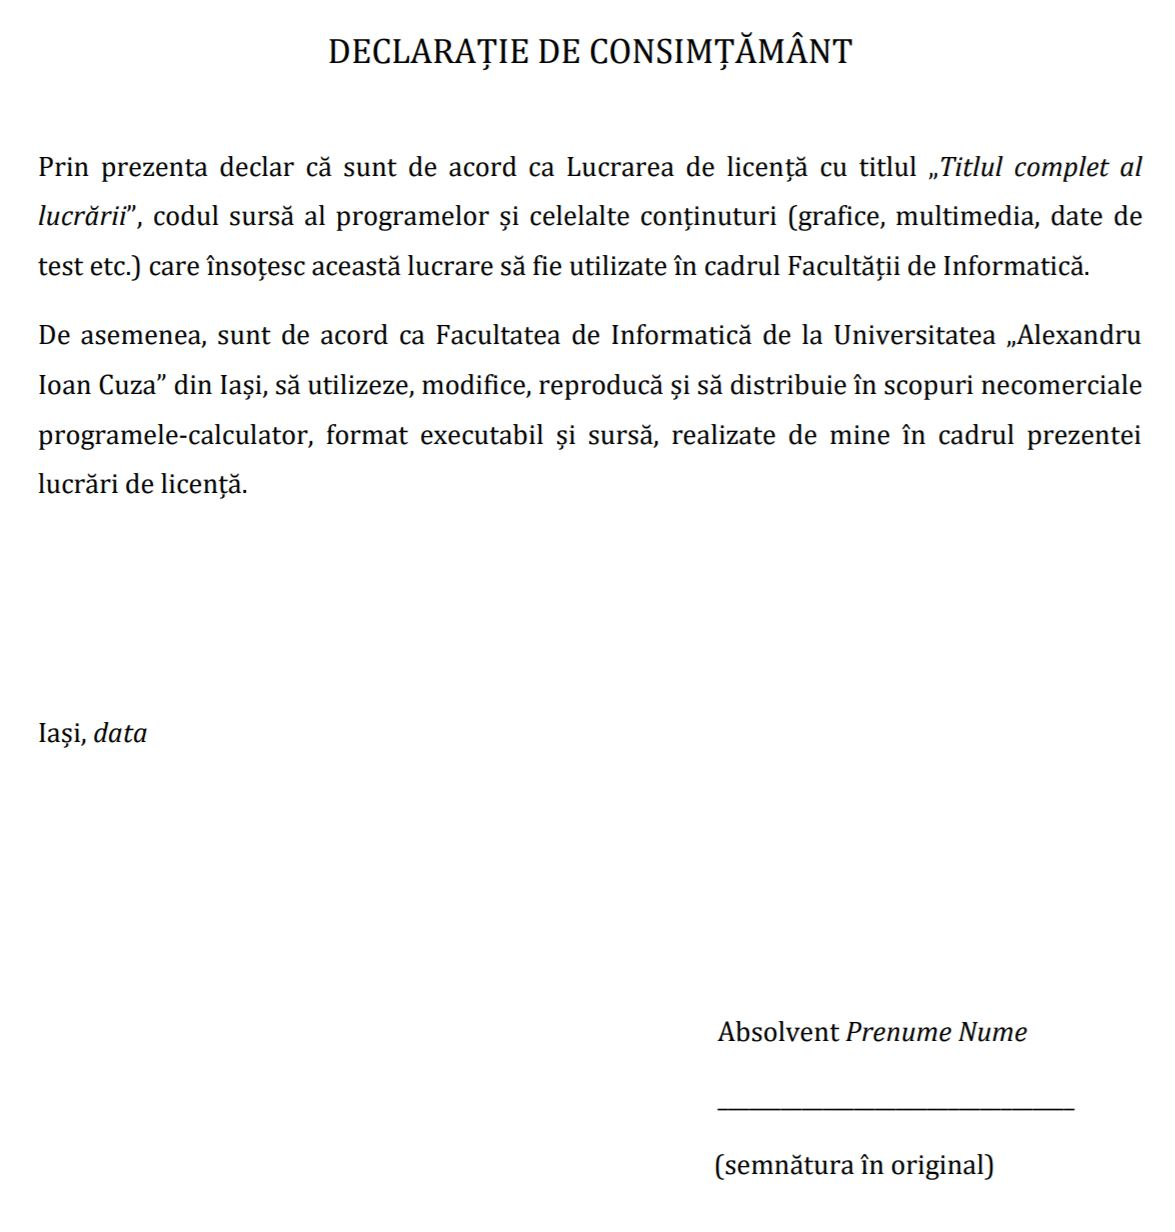
\includegraphics[scale=1.1]{anexa5}}
\centerline{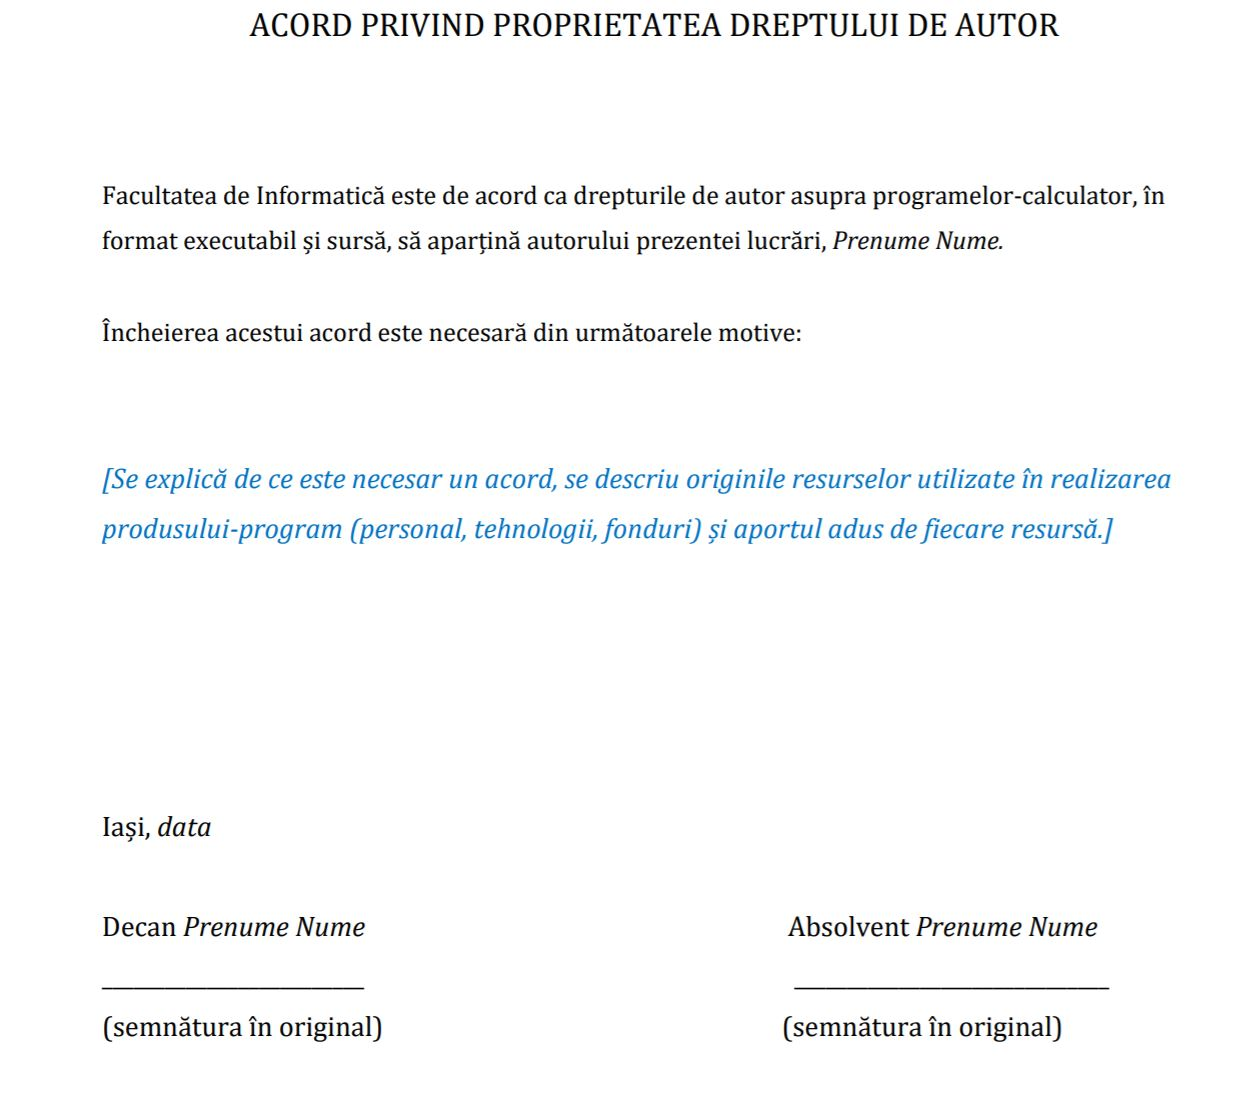
\includegraphics[scale=1.1]{anexa6}}
 \tableofcontents

\newpage
 \section* {INTRODUCTION}
In this current day and age information is available to almost anyone who has access to a network connected device such as a laptop, computer or smartphone. However, although easy to find, depending on the topic of the sought data, some concepts can prove challenging to even the most experienced readers. Scientific papers that contain extensive amounts of numerical data can look very daunting to a first-time reader or even a professional. Subjects such as history, mathematics or biology contain complex details that require memorization in order to be mastered and such things can be very difficult to achieve when the only source of information is represented by paragraphs of text. \par

The concept of using images in order to convey the meaning of data has been around for centuries. From maps curated by famous world explorers to anatomy charts and architectural plans, drawings have proven to be a powerful tool in helping humans understand various topics. This notion is widely known under the name "Data visualization": the attempt of taking textual information and putting it in a visual context in order to simplify it and engage the viewer's visual senses. It is a quick and easy way to convey information and help the reader get a better understanding. It can range from simple bar graphs or pie charts to very complex and artistic videos. \par

\textbf{Timelines} are part of the previously mentioned concept and are visual representations of important events or periods of time in chronological order. Their main purpose is to help the viewer get a better perspective on the progress of historical or modern events or on the life of important personalities. Timelines represent an elegant way of visualizing data and make it easier for professionals to plan, manage and analyze relevant temporal facts. They are very useful in educational fields since they aid in documenting any type of development by providing an easy-to-understand image of past and ongoing trends.\par

\begin{figure}[b]
\centerline{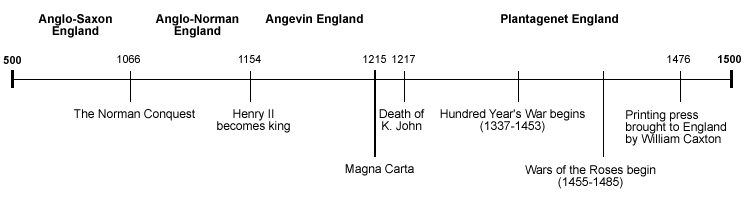
\includegraphics[scale=1.8]{media_timeline}}
\end{figure}

Timelines can be very flexible when it comes to the visual aspect. The most common method of representation is the horizontal approach where numbers, depicting decades, years, months, days, etc. are displayed on an axis. The data to be displayed is usually represented vertically by labeled parallel bars that span over a given time period. This design is popular among companies and is known as a Gantt Chart. It is mainly used to illustrate and plan the progress of a project. The bars in a Gantt Chart show tasks to be performed while the horizontal axis displays the start and finish dates for the aforementioned tasks.\par

While horizontal timelines are perfect for showcasing spans, vertical timelines can be very useful when the data is represented by a single piece of temporal information (one year, one day, etc). Such events include product launches, critical discoveries, the founding of institutions or other important achievements. For example, a vertical timeline would be very useful for showcasing a history of the most important space missions conducted by a space agency.\par

Other timelines make use of more creative design concepts. Designers have taken the freedom to express their creativity when it comes to displaying data in a beautiful and interesting format. Especially in this day and age,  we can see data represented on spiral or serpentine timelines. As long as the data is easy to view and understand there are virtually no limits to designing a timeline.\par 

\begin{figure}[h]
    \centering
    \begin{minipage}{0.5\textwidth}
        \centering
        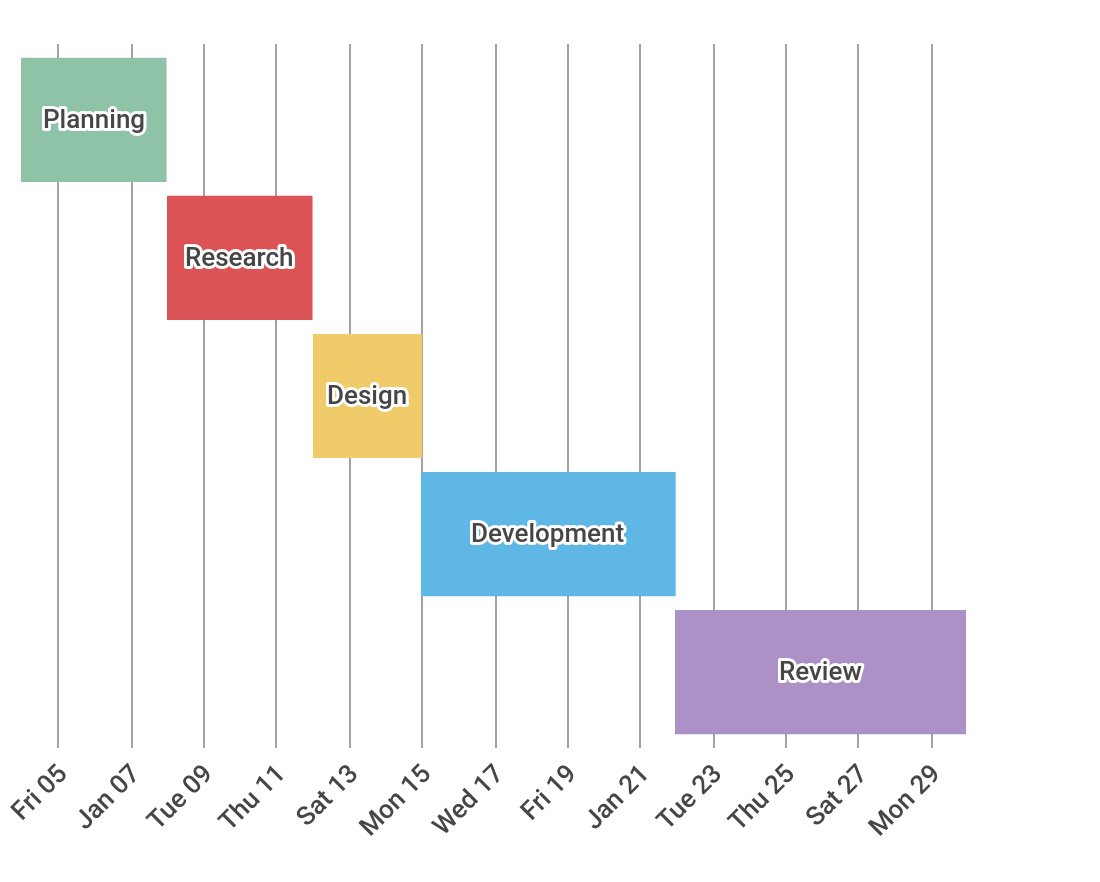
\includegraphics[width=1.2\textwidth]{gantt}
        \caption{An example of a Gantt Chart}
    \end{minipage}\hfill
    \begin{minipage}{0.45\textwidth}
        \centering
        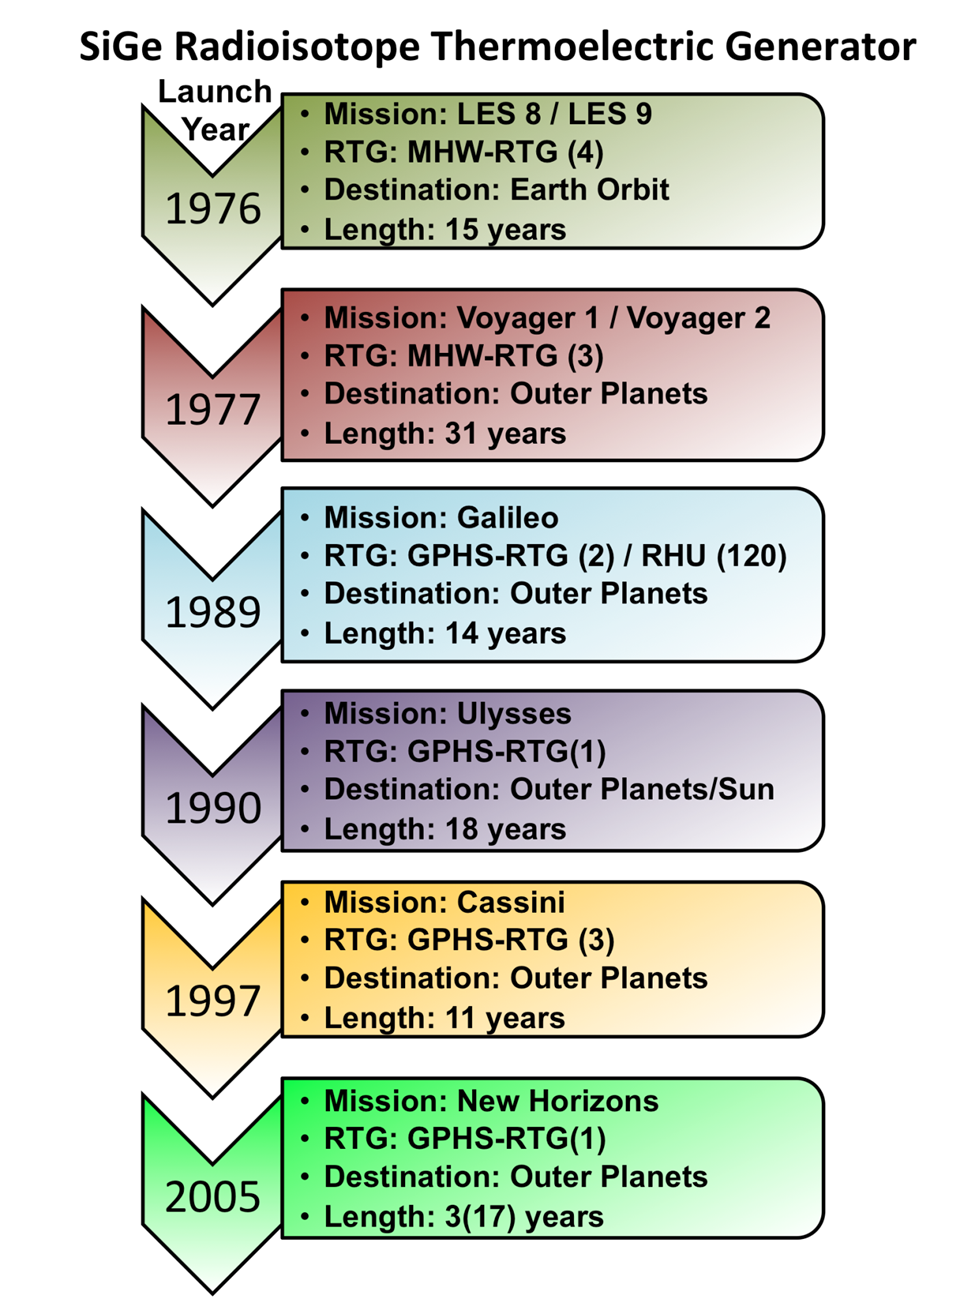
\includegraphics[width=1.1\textwidth]{nasa}
        \caption{An example of a vertical timeline showing space missions}
    \end{minipage}
\end{figure}

People like to see visual representations of any type of information and even more so if it is about themselves. Therefore, in more recent years social media sites have implemented more or less the concept of timelines in order to help their users examine and review their personal data. Notable examples include LinkedIn and Facebook. \par

\begin{wrapfigure}{r}{0.4\textwidth}
	\vspace*{-1.2cm}
    \centering
    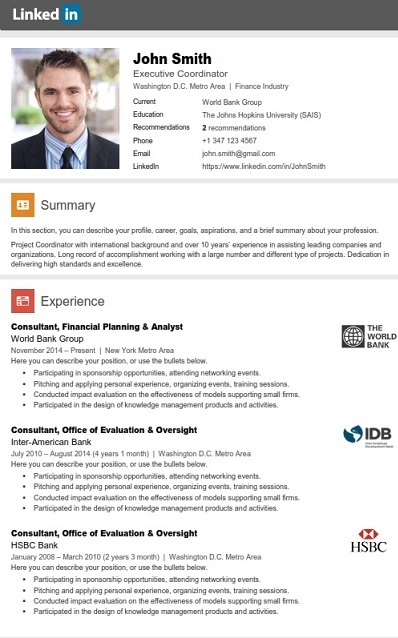
\includegraphics[width=0.5\textwidth]{linkedin}
	\vspace{-80pt} 
\end{wrapfigure}
The LinkedIn platform is a website mainly used for professional networking. The timeline aspect of this service is its ability to allow people to create their CV and update it whenever changes occur. Thus possible employers can easily analyze the career history of users who are looking for a new job.\par

Facebook, the American social media platform, revamped the method of displaying user posts in 2011. Status updates, photos, interactions with apps and events were now displayed in a chronological feed, which bore the name “Timeline”.\par

Despite such platforms using the concept of timelines, they are not focusing too much on the visual aspect of it, thus giving one more reason for an application that deals with such aspects to be implemented.\par

However, it is not only the virtual world that benefits from the usage of timelines. As it has been mentioned before, visual representations of chronological data bring great benefits in educational fields. School manuals, especially History and Biology manuals, make great use of timelines. Young students are more inclined to memorize information displayed in a visually pleasing manner rather than entire paragraphs of text. In universities, professors and students alike use this concept to teach and learn. \par

Given the above-mentioned information, it is clear that timelines make a great and useful tool for a wide range of domains. Thus the topic of this thesis has been chosen in order to provide an application through which a user can easily create a timeline by manually adding events and important real-life or fictional characters or by using a search engine which automatically detects time spans and other useful data for the given input and adds it to the timeline. \par

The target group of this web application mainly consists of people who operate in fields such as History or Linguistics, since their professions involve working with massive amounts of temporal data. However, given the light and intuitive design it possesses, the app can be used by anyone with basic internet skills who wishes to display desired information in chronological order. \par

The thesis is divided into four chapters, each describing a different concept related to the application. \par

The \textbf{first chapter} presents the motivation for choosing to implement the mentioned topic as a web application, as well as the advantages and disadvantages of choosing this environment. \par

The \textbf{second chapter} names the technologies used for the application along with the motivation for choosing them. \par

The \textbf{third chapter} describes in detail the ideas that were used to design the application as well as every functionality it possesses. \par

The \textbf{fourth chapter} focuses on the AI aspect of the project. It describes the general concept of each algorithm and which alterations have been made in order to adapt them to the timeline application. \par

\newpage

\chapter {Topic motivations}

\section {State-of-the-art}

As of 2019, a few applications that deal with generating timelines have been created. Most of them are subscription based and have mandatory registration, requiring a monthly payment in order to gain and maintain full access.\par

TimeGlider is one such application. Events can be recorded by hour, day, month or year, multimedia such as images, video and audio files can be added, and the final result can be shared via accessible URLs. The downsides of TimeGlider are lack of free service and the fact that the manipulation of the eventual timeline can become difficult to master.\par

Tiki-toki is another online timeline maker software. This application encourages a more creative approach as it enables the user to choose different designs and perspectives when creating a timeline. However, just as TimeGlider, Tiki-toki is a very restrictive application for free users, allowing the creation of a single timeline. Subscriptions range from 7.50\$ to 25\$ a month and although very professional and detailed, it does not represent a good alternative for those who cannot afford to pay for a monthly service.\par

TimeToast, TimeRime, Sutori are some other services that implement similar designs and strategies. TimelineGenerator takes inspiration from such applications and uses it in order to develop and offer a free and easy-to-use web application.\par

\section {Web applications: advantages \& disadvantages}

\begin{wrapfigure}{r}{0.4\textwidth}
	\vspace*{-1cm}
    \centering
    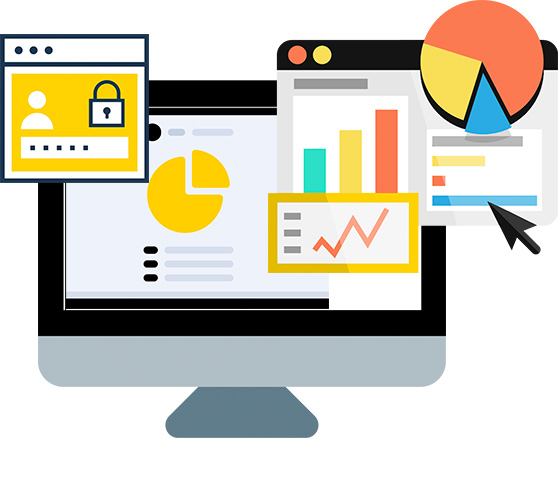
\includegraphics[width=0.4\textwidth]{web}
	\vspace{-10pt} 
\end{wrapfigure}

A web application can be described as any computer program that uses web technologies and a web browser as its client in order to perform a given functionality. Web applications use a combination of server-side (storage and retrieval of information) and client-side (presentation of information) scripting languages in order to be developed. They represent a popular choice for many developers as they do not require the construction of a client and are not OS specific, an internet connection and an installed browser (features which are present on almost every computer nowadays) being the only requirements for such an application to run, in contrast with classic desktop applications, which require installation on a local computer. \par 

Web applications are cost-effective when it comes to troubleshooting and development. Although the user interaction with the graphical interface requires testing on different browsers, the back-end part of the application does not require compatibility with other operating systems versions or configurations. Since they require constant internet connection, applications give users the ability to do remote work. \par

However, there are some downsides to web applications that must be taken into consideration when choosing this environment. Despite the vast array of functionalities available on a web application, all of them require an internet connection which, when slow, turns into a disadvantage as it leads to longer waiting times and sometimes failures. Lack of internet connection altogether means that the application cannot be accessed at all. The fact that an application has to be tailored in order to fit every popular browser can be considered a disadvantage as well. \par

Web-based applications come with an extensive list of advantages that outweigh the disadvantages. They are easy to use and develop, updates are instant on every device, sometimes require no installation and are a very secure option for users as well as developers. \par

\begin{figure}[b]
\centerline{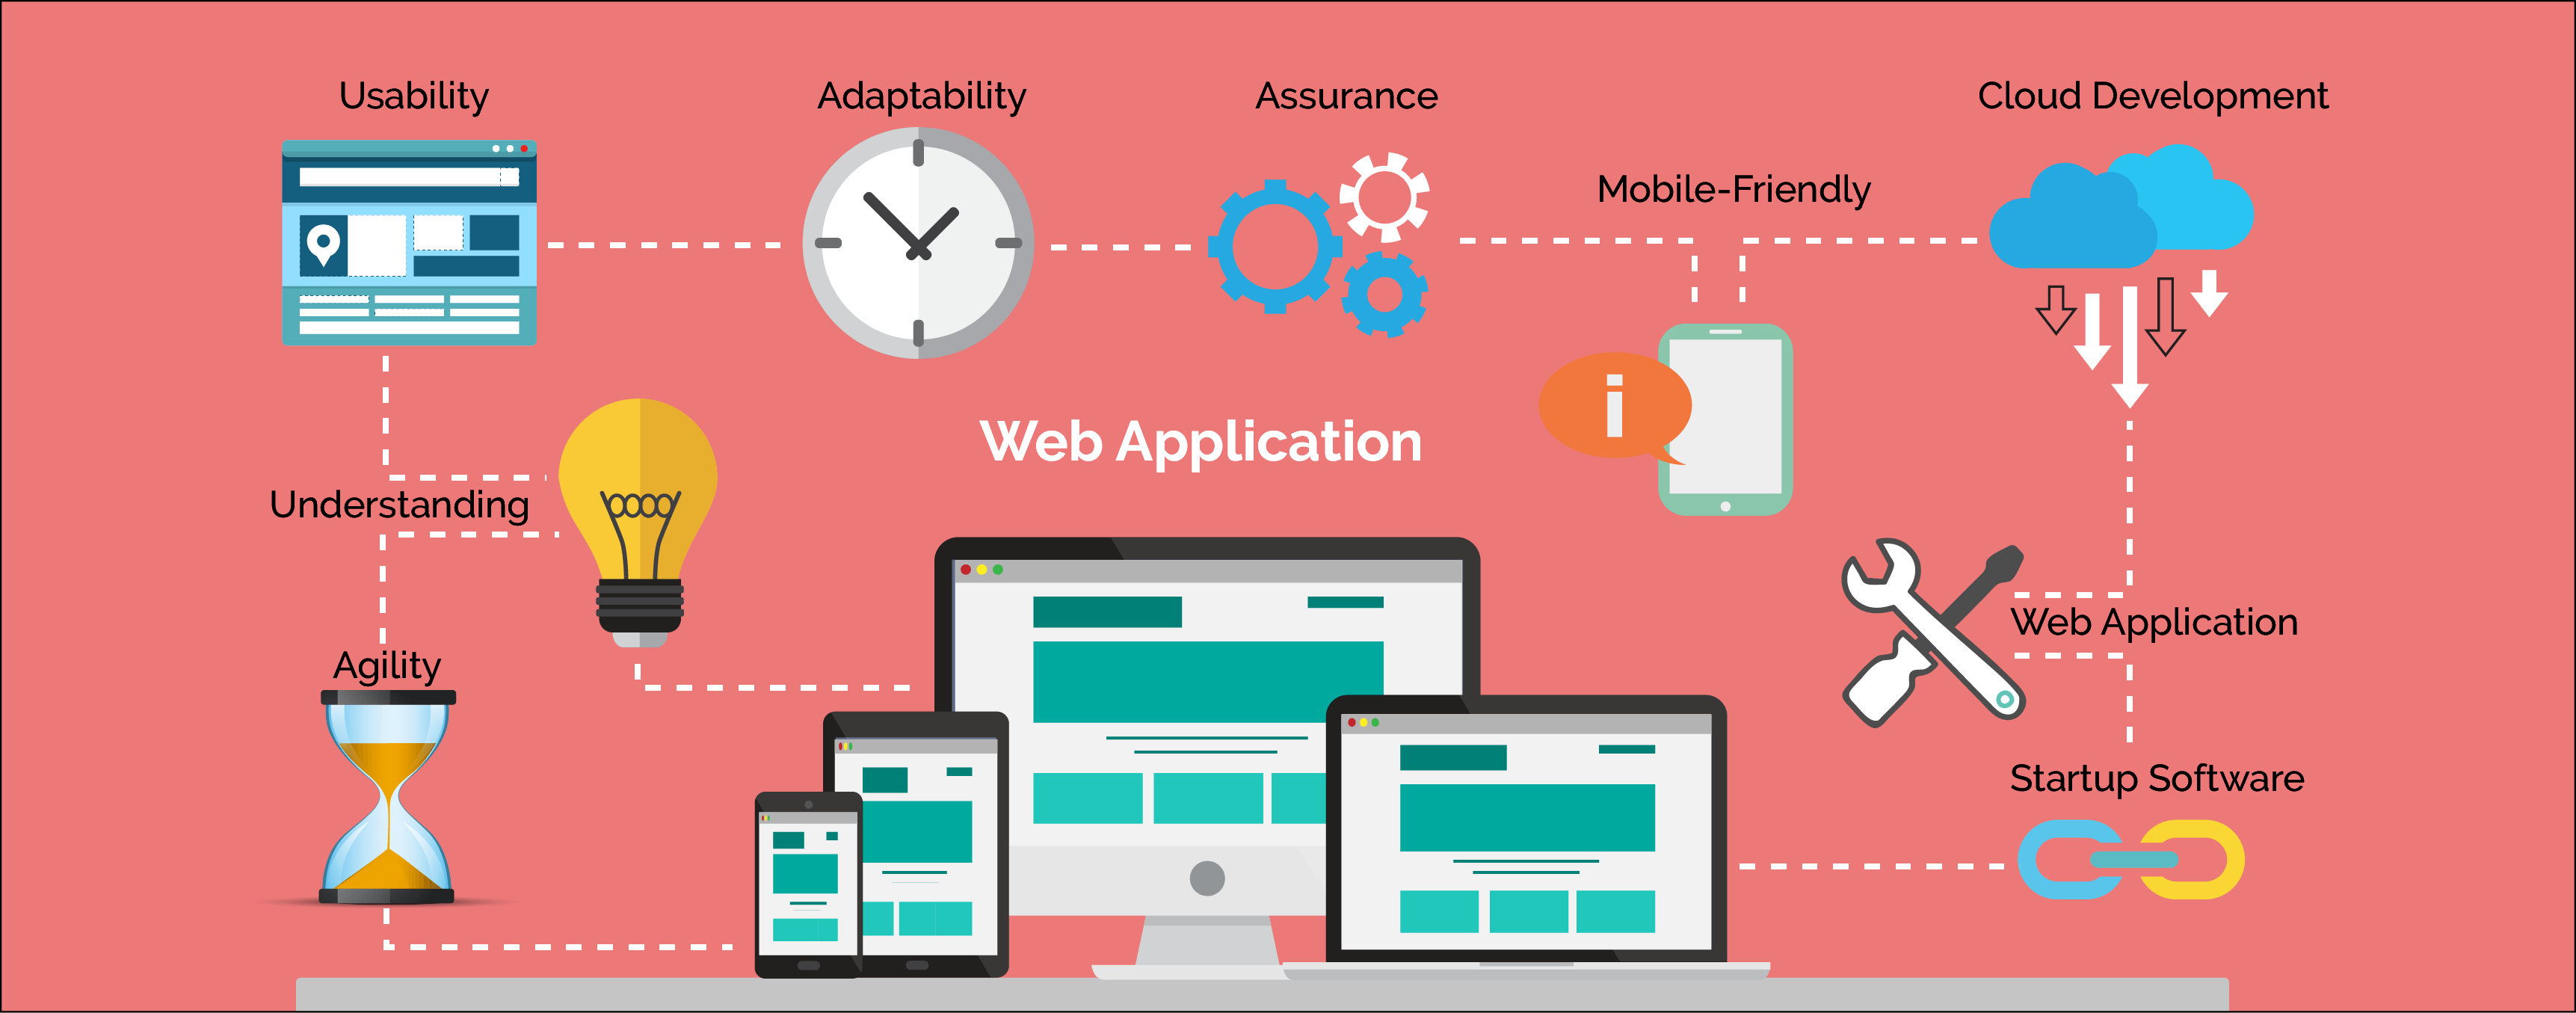
\includegraphics[scale=0.1]{webapp}}
\end{figure}

The main purpose of the TimelineGenerator application is to allow a user to display temporal data in a simple, easy-to-read manner. Although many programming languages provide the ability to create a graphical user interface, very few of them are aesthetically pleasing, fully customizable and well documented. The Java Swing GUI widget toolkit, as well as the TKinter module for Python, have both been considered in the beginning as methods for creating the application. But although very popular, they present a very rigid, old-fashioned display which is not ideal when it comes to data visualization. \par

In recent years web applications have evolved from simple static pages created using only basic HTML to incredibly complex applications that incorporate many features. This is possible nowadays because of the existence of CSS and Javascript alongside many frameworks that promote code reuse and are created in order to ease the job of the developer and improve the quality of design. \par

The TimelineGenerator application has made use of already existing libraries and frameworks such as Bootstrap, jQuery, Node.js and Express, the main reason behind it being the popularity. NPM is a package manager for Node.js containing over 800,000 packages written in JavaScrip, including packages that implement AI algorithms, such as the ones needed for the application.

In conclusion, the decision to create an application that generates a timeline based on user input as a web-application was made on the basis of suitability, popularity, and facility. The main goal of the program was to create a fully functional application through technologies that would speed up the implementation process, avoid building from "scratch" and dealing with troubleshooting. \par

\newpage

\chapter {Technologies}

The technology stack represents an important part in the development of a software product. It mainly consists of sets of tools and frameworks that are meant to help the programmer and speed the implementation process. The stack is divided into front-end and back-end components. The following pages will describe each technology one by one in order to provide a better understanding of them and their purpose in the TimelineGenerator application. 
 
\section {Front-End}
Front-end web development also referred to as the “client-side”, converts data into a graphical interface for the user to view and interact with it through digital interaction using HTML, CSS and JavaScript.

\begin{wrapfigure}{r}{0.2\textwidth}
	\vspace*{-1.5cm}
    \centering
    
\includegraphics[width=0.2\textwidth]{bootstrap}
	\vspace{-10pt} 
\end{wrapfigure}

\subsection {Bootstrap}
Perhaps one of the most popular HTML, CSS and JS frameworks, Bootstrap is a free-to-use, open-source, comprehensive library created for designing responsive mobile-first web pages. It consists of design templates for navigation, forms, buttons, typography, dropdowns and many other interface components. \par

Originally intended as a blueprint for Twitter, Bootstrap was created and developed by Mark Otto and Jacob Thornton as a framework meant to encourage consistency across internal tools. It comes with several JavaScript components in the form of jQuery plugins. Currently, the framework is at its fourth release, with the fifth one already in development.

\begin{wrapfigure}{r}{0.3\textwidth}
	\vspace*{-1.5cm}
    \centering
    
\includegraphics[width=0.2\textwidth]{jquery}
	\vspace{-10pt} 
\end{wrapfigure}
\subsection {jQuery}
jQuery is a light-weight, feature-rich JavaScript library designed to simplify the HTML DOM tree traversal and manipulation, event handling and animation. jQuery was originally created in January 2006 at BarCamp NYC by John Resig, influenced by Dean Edwards' earlier cssQuery library. Just as Bootstrap, it is a free,  open-source software and is currently used by 78\% of the most popular websites nowadays. \par
jQuery is preferred by a big number of developers since it greatly simplifies DOM manipulation syntax and provides the ability to add event handlers to it instead of the classic HTML event attributes which call JavaScript functions.

\subsection {jscolor}
Jscolor is a self-sufficient JavaScript library consisting of a single JS file, for implementing a customizable web color picker component. Jscolor does not require any framework in order to function properly but can be used in accordance with one. The library is also supported by all modern browsers including Google Chrome, Firefox, Internet Explorer 7 and Safari.


\section {Back-End}
Back-end web development is commonly referred to as the "server-side" and represents the part of a computer system or application that is not directly accessed by the user, typically responsible for storing and manipulating data.

\begin{wrapfigure}{r}{0.4\textwidth}
	\vspace*{-1cm}
    \centering
    
\includegraphics[width=0.3\textwidth]{nodejs}
	\vspace{-10pt} 
\end{wrapfigure}
\subsection {Node.js}
Node.js is a free, open-source JavaScript runtime environment that executes JavaScript code outside of a browser and runs on various operating systems, such as Windows, Linux, Unix, etc. Node.js can generate dynamic page content, execute file operations on the server, collect form data and work with databases. Node.js allows Web servers and networking tools to be created through the use of JavaScript as well as a collection of "modules" that handle various core functionality. The modules use an API designed to reduce the complexity of writing server applications. At a high level, Node.js combines the Google V8 JavaScript engine, a single-threaded non-blocking event loop, and a low-level API for input/output operations. It was created when the original developers of JavaScript extended it from something that could only be run in the browser to something that could run on a personal machine as a standalone application.\par

The architecture of Node.js can be characterized as event-driven and capable of asynchronous I/O operations. Node.js's most significant feature is that its functions are non-blocking, commands executing concurrently or even in parallel, and using callbacks to signal completion or failure. The purpose of these design choices is to optimize throughput and scalability in web applications with many I/O operations, as well as real-time Web applications such as live communication programs and multiplayer browser games). \par
\begin{wrapfigure}{l}{0.4\textwidth}
	\vspace*{-1cm}
    \centering
    
\includegraphics[width=0.3\textwidth]{npm}
	\vspace{-10pt} 
\end{wrapfigure}
Most Node.js libraries are hosted on the NPM website which includes open-source web frameworks such as Express.js, which are meant to accelerate the development of applications. 

\subsection {Express}
Express is the most popular framework for Node.js as well as the underlying library for a great number of other Node web frameworks. It is minimal and flexible and provides a robust set of features for applications on the web as well as mobile platforms. It was released in November of 2010 and is currently on version 4.17.1.\par

Express is an unopinionated type of framework, which means it has fewer restrictions when it comes to the structuring of a project and the methods used in its creation. Express makes it easier for a developer to choose whichever tool they want and also allows them to create the directory structure.\par

The framework provides methods through which the user can specify what function is called for an HTTP verb and URL pattern, as well as methods that specify the template engine that is in use. Express middleware can be used for getting POST/GET parameters or if support for sessions, users or cookies is needed.

\subsection {body-parser}
Body-parser is a middleware for Node.js which parses incoming request bodies before the handlers. Body-parser is required in order to handle HTTP POST requests in Express.js version 4 and above. It extracts the whole body portion of an incoming request and makes it available under the \textit{req.body} property. The module can parse strings, buffers, JSON and URL encoded data. 

\begin{wrapfigure}{r}{0.4\textwidth}
	\vspace*{-1cm}
    \centering
    
\includegraphics[width=0.3\textwidth]{mediawiki}
	\vspace{-10pt} 
\end{wrapfigure}
\subsection {MediaWiki action API}
The MediaWiki action API is a web service that grants user access to Wikipedia features such as authentication, search and page operations. It is an unofficial API but since Wikipedia is built using MediaWiki, which supports an API, Wikipedia does as well. It focuses on high-volume use cases and is tightly integrated with the MediaWiki globally distributed caching system. It provides code-level access to entire Wikipedia references and it is mostly used by extension developers, Wikipedia site administrators, and third-party developers.

\subsection {Cheerio}
The Cheerio module is a fast and flexible implementation of jQuery syntax, designed specifically for the server. It allows the developer to scrape web pages by parsing the markup language and providing an API which traverses and manipulates the data resulting from the given URL. Cheerio does not visually render, apply CSS, load external data or run scripts.

\subsection {Compromise}
Compromise is a JavaScript natural-language processing library that interprets, parses and transforms text in the English language. It was designed by Spencer Kyle and meant to be a straightforward way to reuse and throw around text. Methods can be chained together and applied flexibly just as it is possible in the jQuery API. The methods can be run on single words or entire documents. Some of the functionalities offered by Compromise include part-of-speech tagging, finding named-entities, grammar-matching, normalization, and verb conjugation. 

\begin{wrapfigure}{r}{0.4\textwidth}
	\vspace*{-1.5cm}
    \centering
    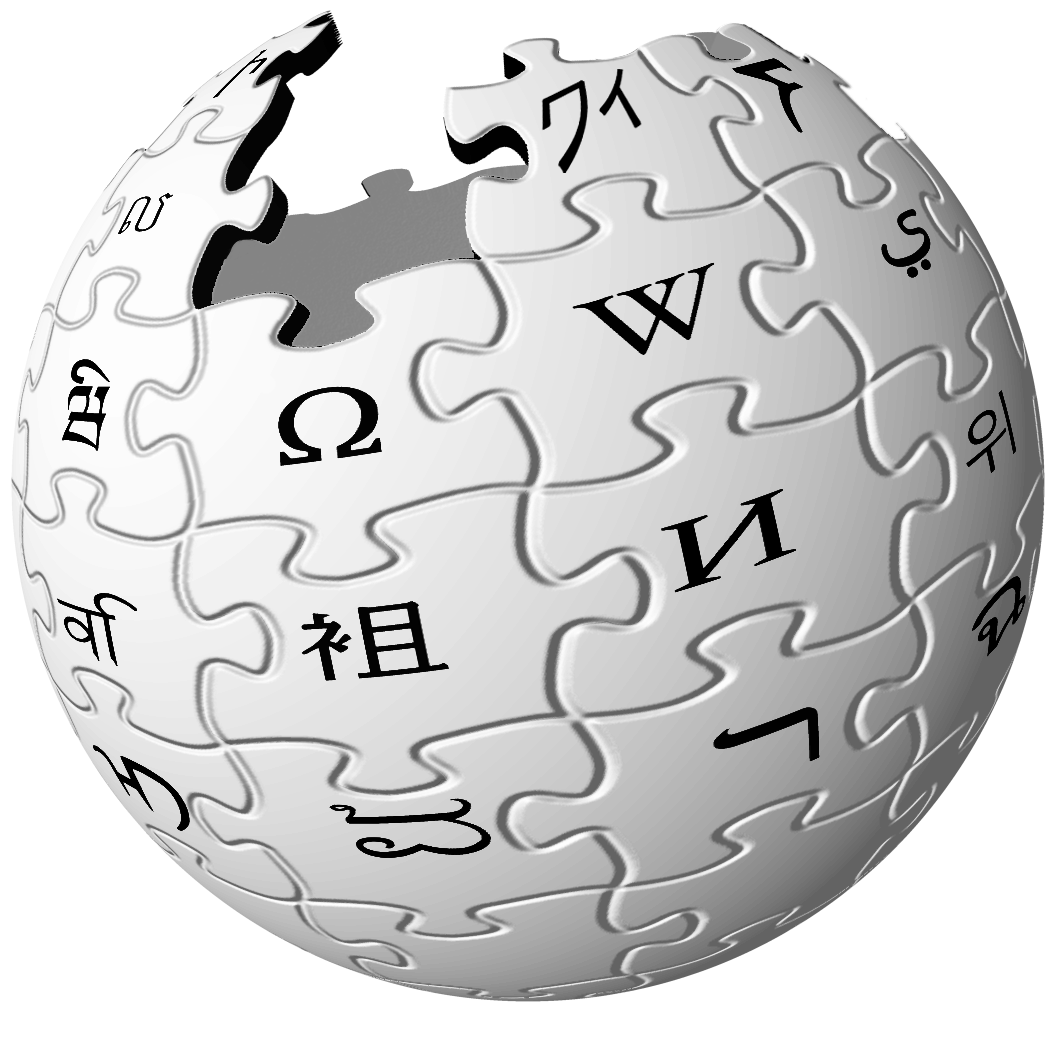
\includegraphics[width=0.3\textwidth]{wiki}
	\vspace{-10pt} 
\end{wrapfigure}
\subsection {WTF\_Wikipedia}
WTF\_Wikipedia is a JavaScript library created by Spencer Kyle with the intent to transform the Wikipedia specific markup-language intro JSON. Considering the fact that Wikipedia pages do not respect a specific template, extracting data from a page can prove extremely difficult. WTF\_Wikipedia can detect redirects and disambiguation pages, parse infoboxes into formatted key-value objects as well as images, headings, and categories.

\textbf{Conclusion}: The technology stack represents a crucial part in the development of an application. Each of the aforementioned technologies has played an important part in the development of the TimelineGenerator application whether or not they were used more or less than others. The frameworks and library have both helped speed up the building process and have caused minor and easy to solve troubleshooting episodes, thus achieving the main purpose of a technology stack.

\begin{figure}[h]
\vspace*{3cm}
\centerline{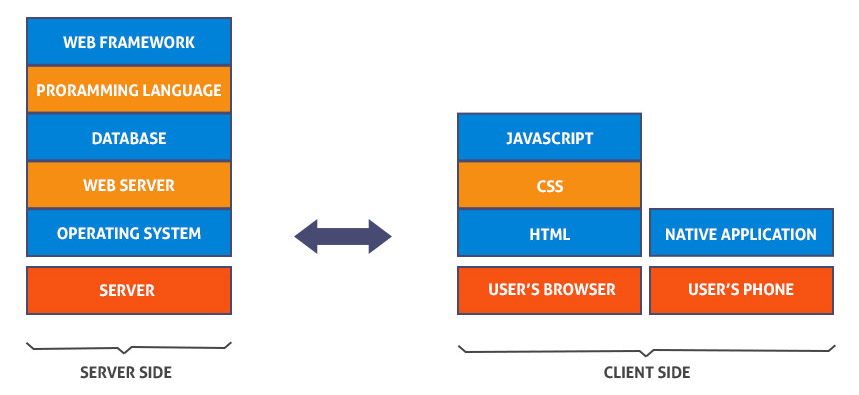
\includegraphics[scale=0.4]{stack}}
\end{figure}
\newpage

\chapter {Ideas \& functionalities}

The purpose of the TimelineGenerator application is to allow any user to create a visual representation of temporal data, whether that consists of life spans, duration spans or simply, dates. The functionalities present on the graphical interface are easy to understand and execute and the design aspect of the timeline is minimalist in order to avoid the visual cluttering of data.\par

The following two sections describe in full detail the ideas and functionalities that were used in order to achieve the final result of the project:

\section {Front-end}
\subsection {Design ideas}
Typical page elements such as buttons, forms, and dropdowns were created using the Bootstrap framework. The colors were kept to a minimum in order to maintain a classic look. \par
A unique component present in the application is the timeline section of the page. This element contains several members bearing the following names in the front-end code of the project:
\begin{enumerate}
  \item \textbf{Year Axis}: numbers representing years are enumerated according to the user's preference. They can be either displayed consecutively or only the years divisible by 5, 10, 50 or 100 in order to keep the axis more compact (the number chosen to divide by is called a \textbf{step}). The years and their corresponding axes are spaced according to the width of the screen when there are less than 42 years to display. The width is divided by the number of years and thus a \textbf{unit} is obtained. When this number is exceeded, the unit takes the constant value of 2.5rem in order to expand the width of the timeline and save the page from looking too cramped. 
  \item \textbf{Bar}: bars represent spans or durations. Their lengths are computed using the \textit{unit} mentioned above and the formula:\\\centerline{\textit{(end\_of\_span - start\_of\_span) / step * unit}}
\end{enumerate}

\begin{figure}[h]
\vspace*{3cm}
\centerline{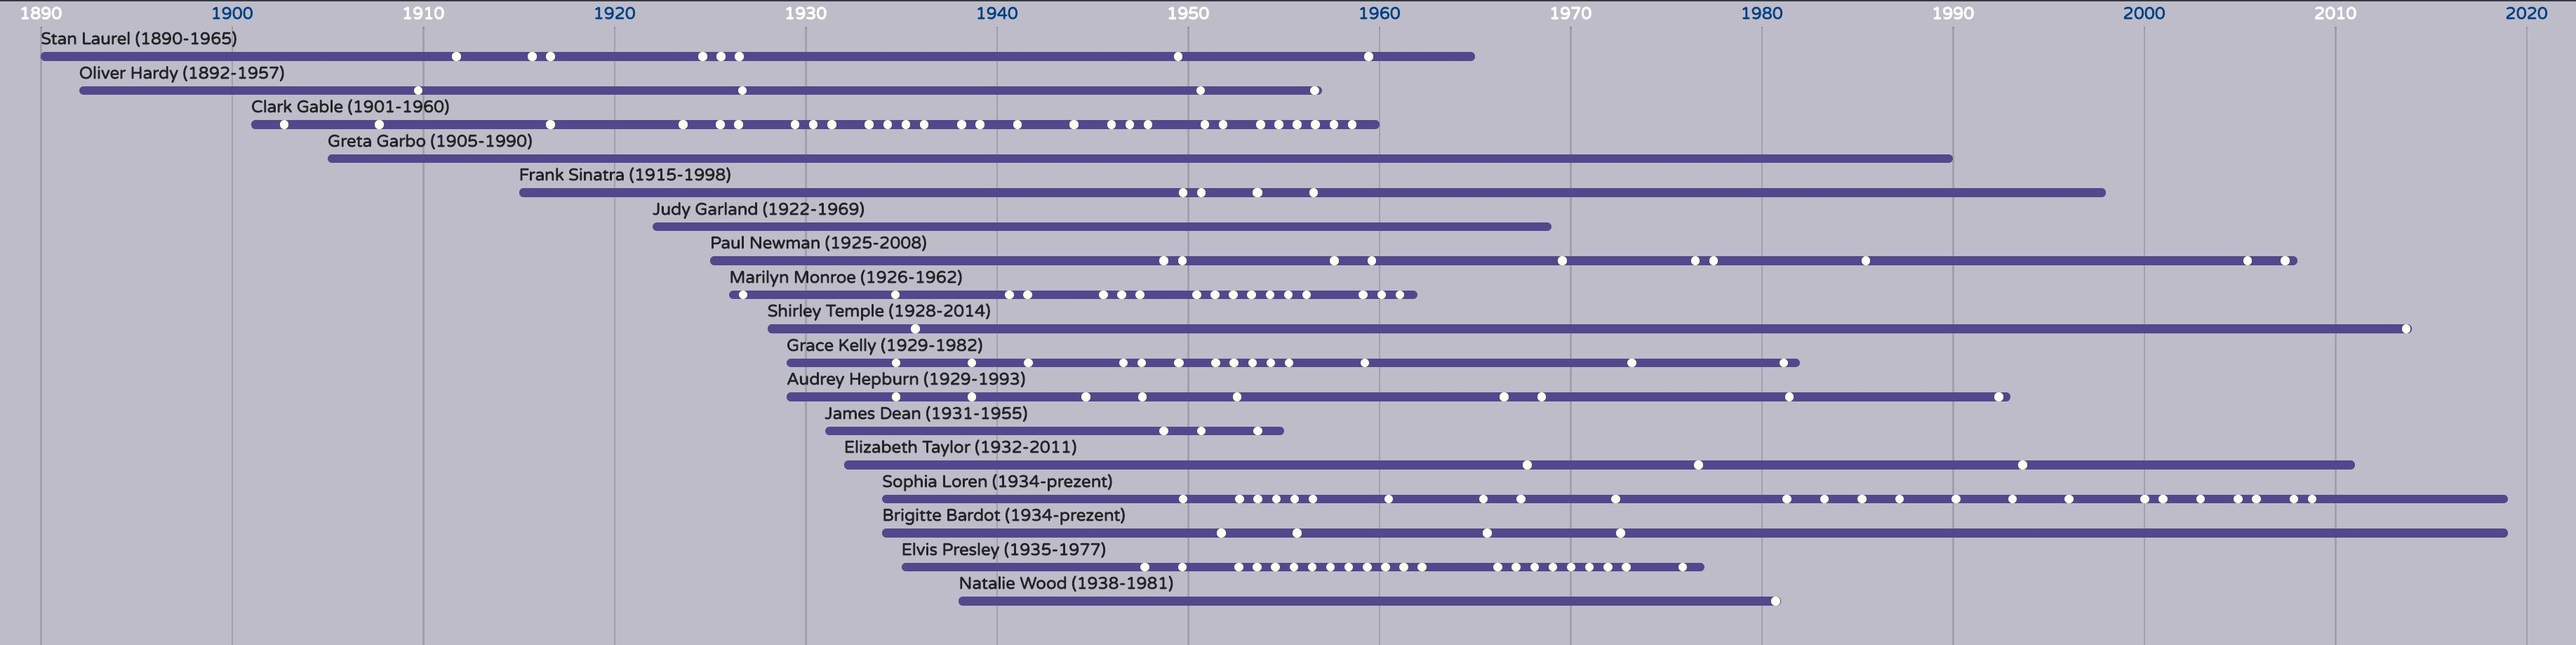
\includegraphics[scale=0.45]{tl}}
\caption{A timeline of famous Hollywood actors and actresses created using TimelineGenerator}
\end{figure}
\newpage
\subsection {Functionalities}
\begin{enumerate}
  \item \textbf{Step}: a drop-down list that allows the user to select how the year axis will be displayed. The default value is 10, meaning that after adding one element, the axis will only show years divisible by 10. Other options include displaying every 1, 5, 50 or 100 years;
  \item \textbf{Add element}: a drop-down form which prompts the user to input desired data (\textit{Figure 3.1}). The fields present in the form are \textit{Image URL}, \textit{Name}, \textit{Occupation}, \textit{Years} and \textit{Description}. The only mandatory field are \textit{Name}, \textit{Occupation} and \textit{Years}. In case no image URL or description is provided, a default picture will be used, and the uncompleted field will remain empty. After an element is added, the Step option becomes unavailable;

  \item \textbf{Search}: the search field allows the user to look for filtered Wikipedia results with the help of the MediaWiki API. Acceptable results are represented by Wikipedia articles which describe events, individuals, releases, etc. and are displayed in a modal. A result in the modal contains the name, a short description, and an image, if available (\textit{Figure 3.2});

  \item \textbf{Add search element}: the add button available for every entry in the modal automatically adds the result to the timeline together with specific events which can be seen when hovering on the corresponding dots lined up on the span bar;

  \item \textbf{History}: the history button activated a drop-down list which holds every entry that had been made to the timeline. The reset button does not delete the history. The history resets itself only when the page is reloaded;

  \item \textbf{Reset}: the reset button resets the variables used in the front-end script and deletes everything that has been added to the timeline section, including the years. The Step option becomes available again when the reset button is pressed.
\end{enumerate}

\section {Back-end}
The purpose of the back-end script is to create an HTTP server and handle the \textit{search} functionality mentioned in the front-end section.\par

\textbf{POST method}: The code uses a \textbf{POST} request to handle the search input. The input is formatted in a way that respects the URI scheme. Thus spaces are replaced with \textit{\%20} (For example if the input is \textit{Alber Einstein}, it will be converted to \textit{Albert\%20Einstein}. \par

Next, the Wikipedia API endpoint is used. The endpoint is the address of the desired data, and Wikipedia allows its results page to be displayed either in XML or JSON format, depending on the needs of the developer. The URL specified in the MediaWiki documentation is used together with the search input to create the full link. Thus the following string will be created in case the search input is \textit{Albert Einstein} :\\\\\centerline{https://ro.wikipedia.org/w/api.php?action=opensearch\&format=json\&search=\textbf{Albert\%20Einstein}}.\par Notice the \textit{ro} in the URL. Since Wikipedia is available in several languages and the TimelineGenerator application is supposed to provide results in Romanian, the original form of the URL has been changed from \textit{en.wikipedia} to \textit{ro.wikipedia}.

Afterward, the \textbf{Cheerio} module is used to load the HTML of the provided URL. The function \textit{cheerio.load(HTML)} loads the HTML from the URL given as a string earlier. Since the parameter \textit{format=json} is present in the string, the html will be displayed in the given format. The following steps are added in order to process the result. The method \textit{\$('body').html()} strips the string off of the html tags, leaving only the following text:\\

    ["Albert Einstein",
    ["Albert Einstein"],
    ["Albert Einstein (n. 14 martie 1879, Ulm – d. 18 aprilie 1955, Princeton) a fost un fizician teoretician de etnie evreiască, născut în Germania, apatrid din 1896, elvețian din 1899, emigrat în                 1933 în SUA, naturalizat american în 1940, profesor universitar la Berlin și Princeton."],
    ["https://ro.wikipedia.org/wiki/Albert\_Einstein"]]\par

The data is then transformed into a valid JavaScript object by using the function textit{JSON.parse(result)} in order to make the process easier and quicker by having accessible lists and values. If the second list of the object is empty, it will be sent to the client and the modal responsible for showing results will display a message for nothing found (\textit{Nu am gasit nimic}).\par

Next, using the \textit{Compromise} library, the result list is refined to contain only suitable options. Compromise provides the function nlp(text).people().out('text') which extracts proper nouns after the given text is processed by an NLP algorithm. To ensure better results, the refined list is filtered once again and entries such as names of geographical locations or general topics are eliminated.\par

The WTF\_Wikipedia library is then used on each remaining element to extract select information from the infobox, if available. The infobox is a fixed-format table which contains summarised information for the topic and can be found in a great majority of Wikipedia articles. The image path, type of result (person, event, unknown) and dates of birth, death, opening, closing, disbandment, etc. will be added to lists in the JSON object or omitted and replaced by default values if not available. The final list will be forwarded to the client to be displayed in the search modal.\par


\textbf{GET method}: A GET request is used by the application when the user adds an element from the search result to the timeline. This is where events are extracted from the Wikipedia article and added to a list that will then be used by the fron-end script to render each event as an entry on the span bar.\par

The method receives through the req parameter the name of the result selected to be added to the axis. The \textit{WTF\_Wikipedia} library is used once again but this time to fetch and store the text contents of the page with the name given by the aforementioned parameter. In order to identify the events in a text, the following regex is used:\\
\verb/(\d{1,2}) (ianuarie|februarie|...|decembrie) (\d{4})|(\d{4})/gi\\
It searches for every sentence which contains a year using the flags \textit{g (global)} and \textit{i (case insensitive)}. In order to identify sentences, they are characterized by sequences of letters, numbers, and spaces in between two full stops. This requirement is not true in 100\% of the cases and meaning that the invalid sentences will be excluded by a filtering function. Some examples of exceptions include grammatically correct sentences which include abbreviated words (\textit{e.g. etc., U.S.A.}) or names that use initials (\textit{e.g. George W. Bush}), both meaning that additional full stops are present without signifying the end of the sentence. \par

Once a correct sentence is found, it will be appended to a newly created JavaScript object as follows: years will be used as keys with values of type list containing every event corresponding to the year key. The final object will then be sent back to the client.\par

\textbf{Conclusions:} The front and back-end design and functionalities work together to create a simple yet effective application for visual rendering and managing of temporal data. The GUI presents a minimalist layout that can be used with ease by anybody in order to achieve the desired results.

\begin{figure}[b]
        \centering
		\vspace*{-3cm}
        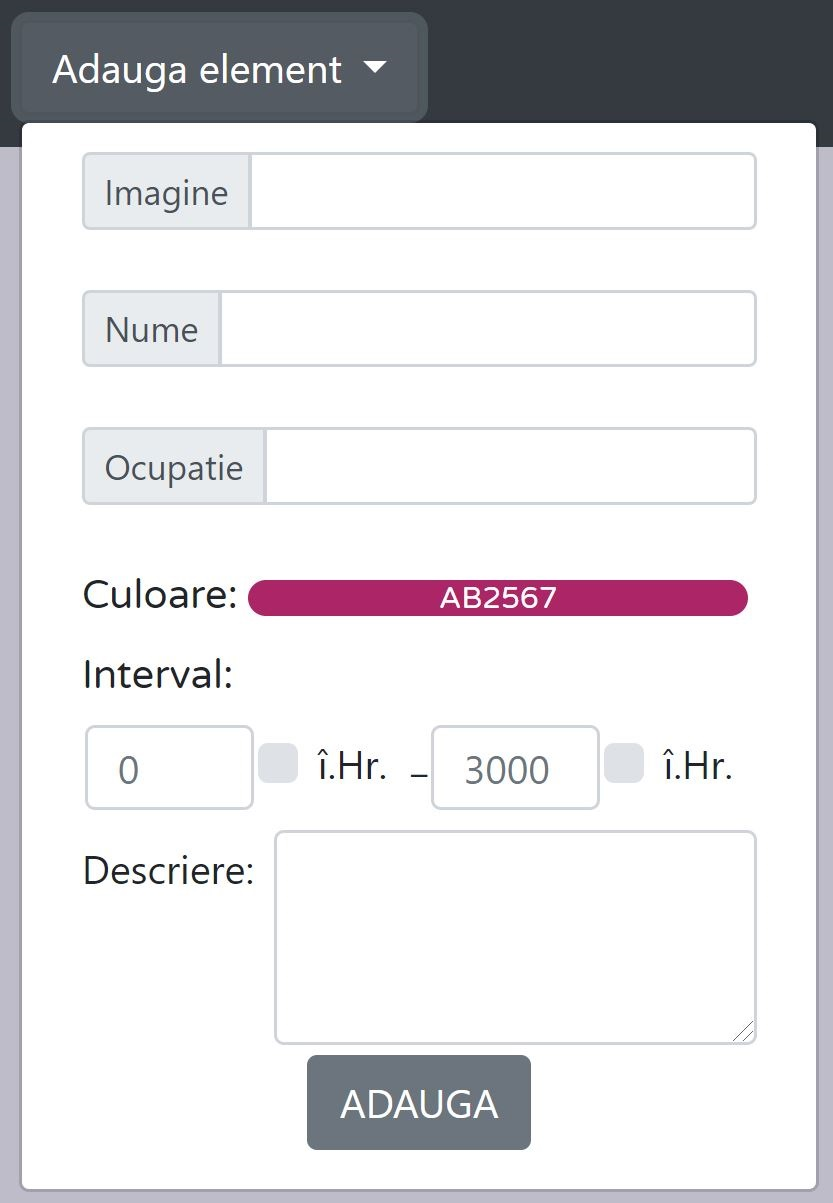
\includegraphics[width=0.6\textwidth]{addbtn}
        \caption{Add element drop-down}

        \centering
		\vspace*{1.5cm}
        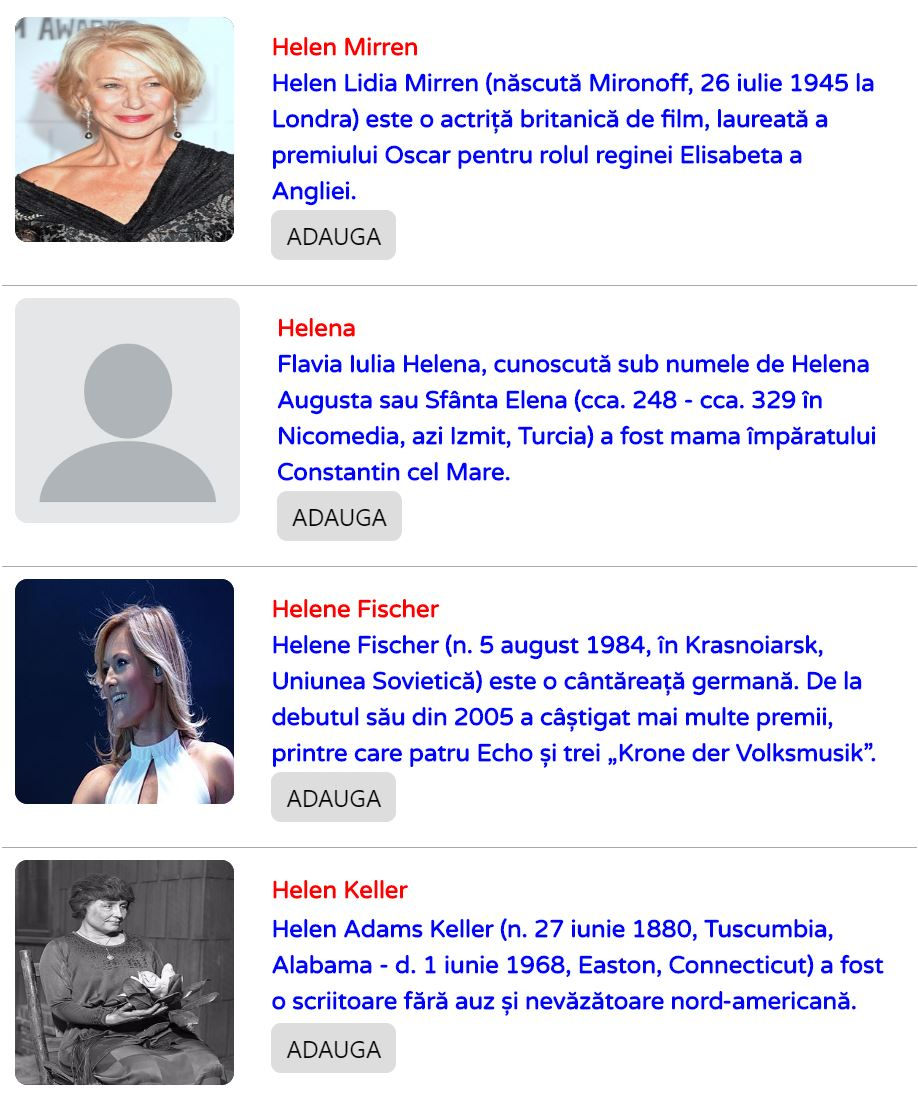
\includegraphics[width=0.6\textwidth]{helen}
        \caption{Search modal showing result for \textit{Helen}}
\end{figure}

\newpage

\chapter {Artificial intelligence concepts and algorithms}

Artificial Intelligence is a branch of computer science which deals with the simulation of human intelligence processes by computer systems by using complex algorithms. Machines can often mimic human behavior if a necessary volume of relevant information is present. As of today artificial intelligence, in short, AI can be seen in various gadgets and online spaces such as search engines, shopping recommendations, and digital assistants. AI technologies are brilliant at analyzing vast amounts of data to learn to complete a particular task, a technique widely known as \textit{machine learning}. \par

\begin{figure}[b]
\centerline{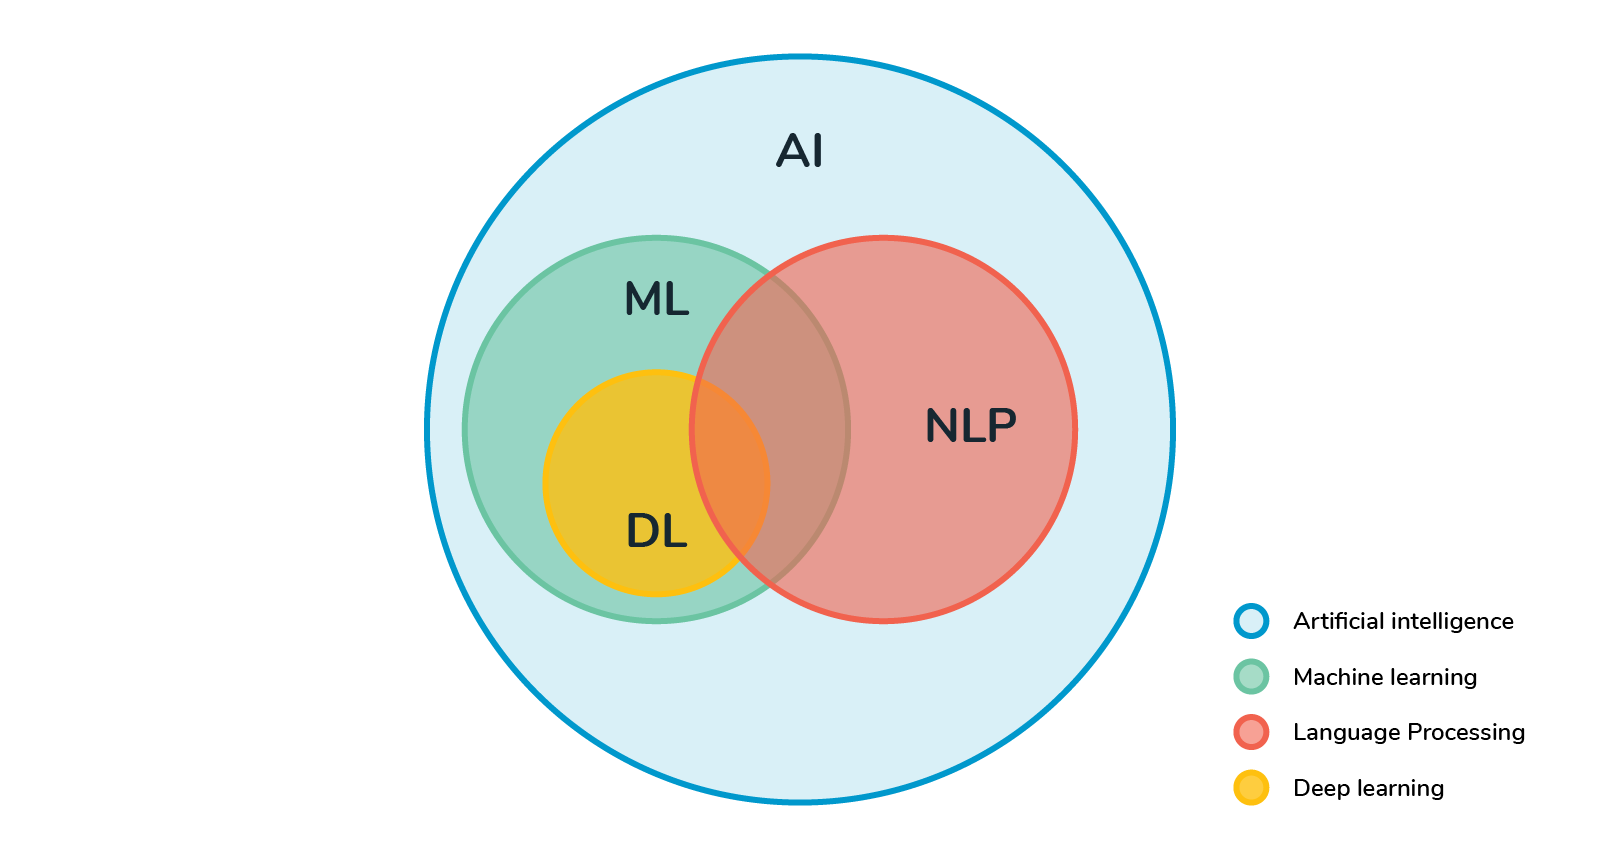
\includegraphics[scale=0.16]{ai}}
\end{figure}

A core part of artificial intelligence, \textit{machine learning} was developed with the intent to make computers learn, reason and self-correct with or without any kind of supervision. Akin to the early stages of human intellectual development, pattern recognition, classification, and numerical regression have become staples in the training of computerized systems. \par

AI can be of two kinds: \textit{weak} and \textit{strong}. Designed and trained for a small range of interconnected tasks, \textit{weak AI} can be seen in virtual personal assistants such as \textit{Amazon's Alexa}, \textit{Samsung's Bixby} and \textit{Apple's Siri}. \textit{Strong AI} is more similar to human cognitive abilities and is built to be able to find solutions when presented with new or unknown situations without manned intervention.\par

The TimelineGenerator application does not delve too deeply into the development of artificial intelligence algorithms but makes good use of some of the most popular ones in order to provide a tool with small and simple smart features. TimelineGenerator uses natural language processing for filtering results and methods of temporal information extraction for event selection. In order to get a better understanding of each concept, they are presented in a clean manner, with concrete examples encountered in the process of building the project.

\section{Natural language processing}
\begin{wrapfigure}{r}{0.4\textwidth}
	\vspace*{-1.5cm}
    \centering
    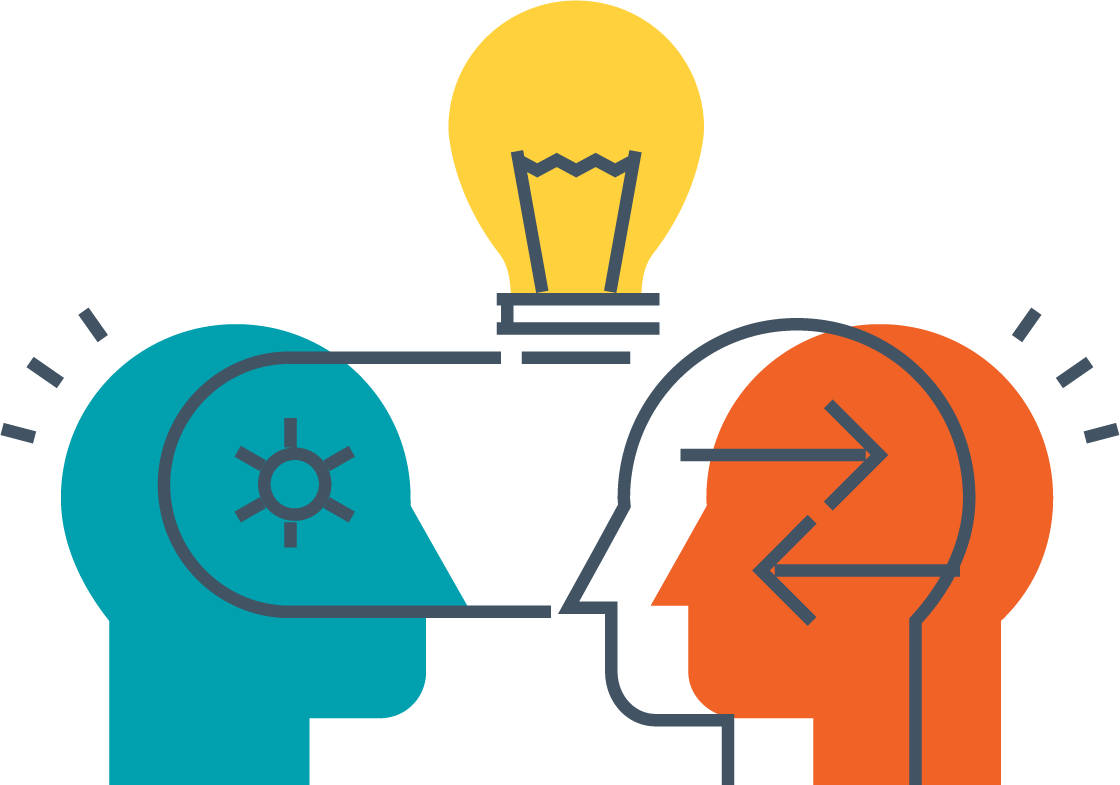
\includegraphics[width=0.3\textwidth]{nlp}
	\vspace{-10pt} 
\end{wrapfigure}
Human beings are the most advanced species on earth and this achievement is mainly due to the ability to communicate verbally and nonverbally in order to share information. The human language is one of the most diverse and complex parts of mankind considering that a total of 6500 languages exist.\par

Natural language processing is a branch of artificial intelligence meant to help computers understand, interpret and operate on the human language in order to fill the gap between humans and machines. While not a new science, it is a rapidly advancing technology thanks to the high-interest rates in the field, the availability of big data and powerful computing algorithms. NLP has many applications and can be found in common web services such as language translation applications (\textit{Google Translate}), word processors that check text accuracy (\textit{Grammarly, Microsoft Word}), personal assistants (\textit{Cortana, Alexa, Siri}) or interactive voice response applications used in call centers. \par

Language processing can prove to be a difficult task, the main cause being the complexity of human languages. Computers use what is known as \textit{machine language} or \textit{machine code} in order to function, a language largely incomprehensible to most humans. Natural vocabulary has to be converted into machine language for it to be understood by computerized systems. Rules for passing information from one human to another vary from basic to high-level and abstract. It is almost impossible for a machine to detect sarcastic tones or emotions in spoken or written language. \par

NLP works by extracting, examining and applying patterns in accumulated data. Computers nowadays are improving their understanding of human languages and their complexities. To speed up the process of analysis, experts make use of several traditional linguistic fields including morphology, syntax, semantics, pragmatics, and phonology. Algorithms can be used to extract the meanings of sentences, tokenize them into parts of speech, extract terminologies, etc. \par

Natural language processing represents a major supporting part in the development of human and machine interactions and as more research is carried and discoveries are made the field is expected to produce smarter machines, capable of recognizing and understanding human communication perfectly.
\begin{figure}[h]
\vspace{2cm}
\centerline{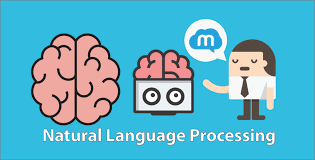
\includegraphics[scale=0.8]{nlp2}}
\end{figure}


\section{Named entity recognition}
\begin{figure}[b]
\centerline{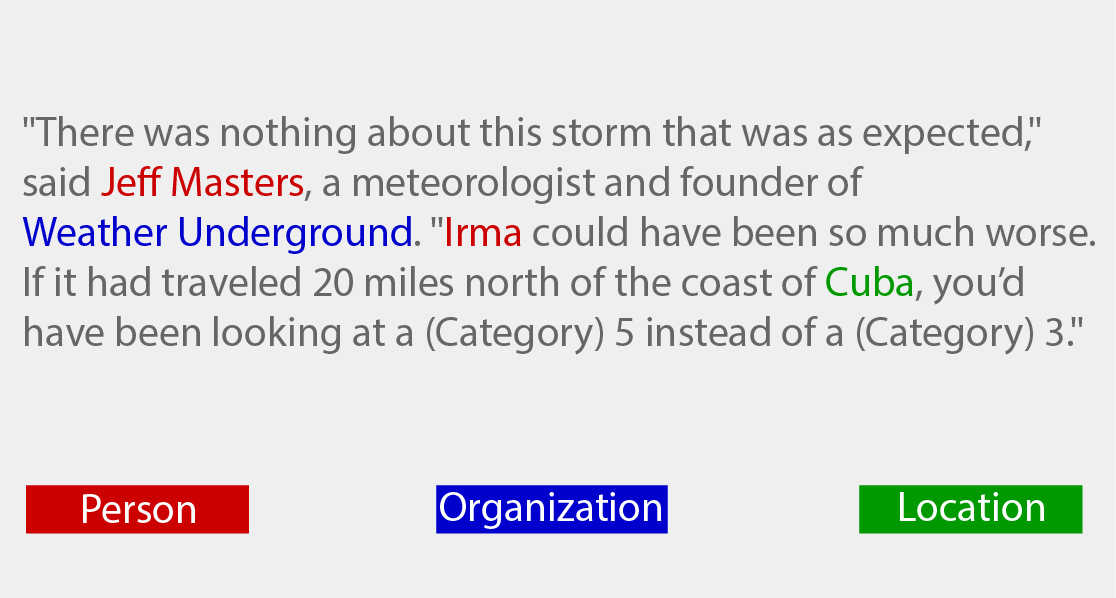
\includegraphics[scale=0.55]{ner}}
\end{figure}
Named entity recognition (\textit{NER}), also known as \textit{entity extraction} or \textit{identification} is a subtask of natural language processing that seeks to identify and classify into pre-defined categories named entities present in a given text. NER adds more substance to scanned data and can aid machines in understanding natural language. \par

In any document, there are bound to be particular words that serve as special entities with more unique context. These terms usually represent people, organizations, places, etc., and denoted by proper names. Full named-entity recognition is divided into two problems: name detection and name classification in accordance with the type of entity they refer to. The first issue mainly refers to a segmentation problem where names are defined as contiguous spans of tokens such that something like \textit{"University of Oxford"} is considered a single name but \textit{"Oxford"} is disregarded as the name of a geographical location because it is contained within the word group. The second issue deals with picking a suitable ontology for the selected word or group of words. \par

NER algorithms have been designed to use linguistic grammar-based techniques and statistical methods. While hand-crafted grammar-based systems can typically obtain better, more accurate results, they require extensive work from computational linguists and cannot be created in a short time. Statistical NER systems, on the other hand, require considerable amounts of training data that has been annotated manually. Semisupervised approaches are a possible solution for avoiding the effort required by annotations. \par

NER can be approached from different domains. There is the classical approach which is mostly rule-based. The machine learning approach centers on treating the problem as a multi-class allocation where named entities are labels to which different classification algorithms can be applied or by using the \textit{Conditional Random Field (CRF)}. \textbf{CRF} is a graphical model that relies on probabilities to model sequential data such as labels of words in a sentence.  Hybrid NERs combine the statistical machine learning with memory-based learning. \par

Named entity recognition is a complex technology with beneficial applications in many areas of study. The approaches for NER are different and have each their own advantages and disadvantages, ranging from rule-based to machine learning and hybrid approaches. Future developments of technologies and algorithms can and will aid in perfecting the NER field as a whole but until then, the already existing methods are powerful tools that can categorize text inputs with accuracy.

\section{Temporal information extraction}
Temporal information extraction is the identification of relational data representing temporal intervals from the unstructured text as well as the extraction and establishment of relations between the items. It is a challenging area of natural language processing research and an essential factor for any system that uses NLP. Information extraction is rapidly gaining more interest from researchers looking to refine knowledge of massive language corpora.\par

\begin{figure}[h]
\centering
\centerline{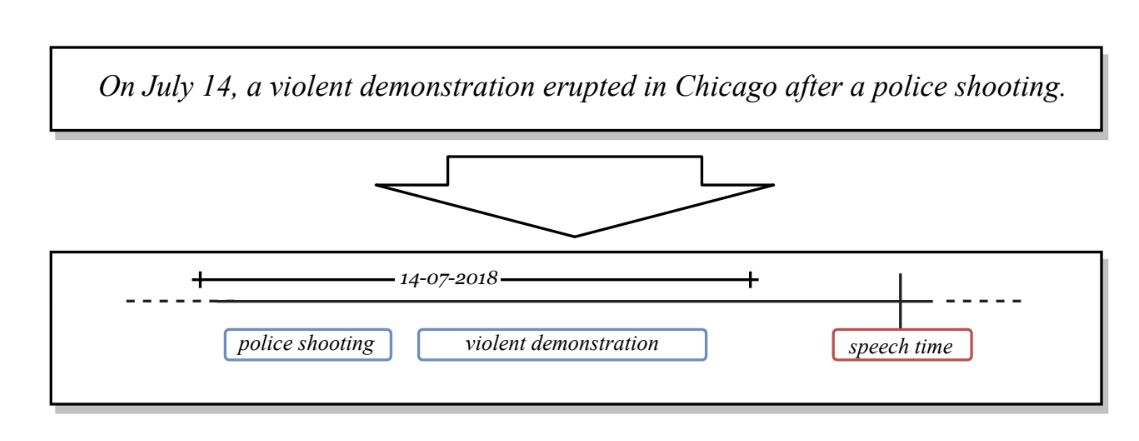
\includegraphics[width=1\textwidth]{tee}}
\caption{Temporal information extraction example (taken from Artuur Leeuwenberg and Marie-Francine Moens' \textbf{A Survey on Temporal Reasoning for Temporal Information Extraction from Text})}
\end{figure}

The current criterion for temporal information extraction is composed of three stages: recognition of events and temporal expressions, recognition of temporal relations among them and time-line construction from temporal relations. \par

The \textbf{Allen interval relations} are a popular framework proposed in 1983 by \textit{James Frederick Allen} in 1983. They are shown in Figure 4.2 and consist of thirteen mutually exclusive basic interval relations that can be assigned to a pair of definite intervals.
Indefinite interval relations can be constructed from these basic relations, which represent connections between exact time intervals, where relative positions of start and end-points are known. For example, the following sentence:\\

\textbf{During breakfast, Jimmy watches the TV. Afterwards, he goes to work}\\

 would be formalized in Allen's algebra as follows:\\

\centerline{\textbf{TV \{d, s, f\} breakfast}}
\centerline{\textbf{breakfast \{\textless, m\} bed}}

\begin{figure}[h]
\caption{Allen's interval algebra rules (Source: Wikipedia)}
\vspace*{1cm}
\centerline{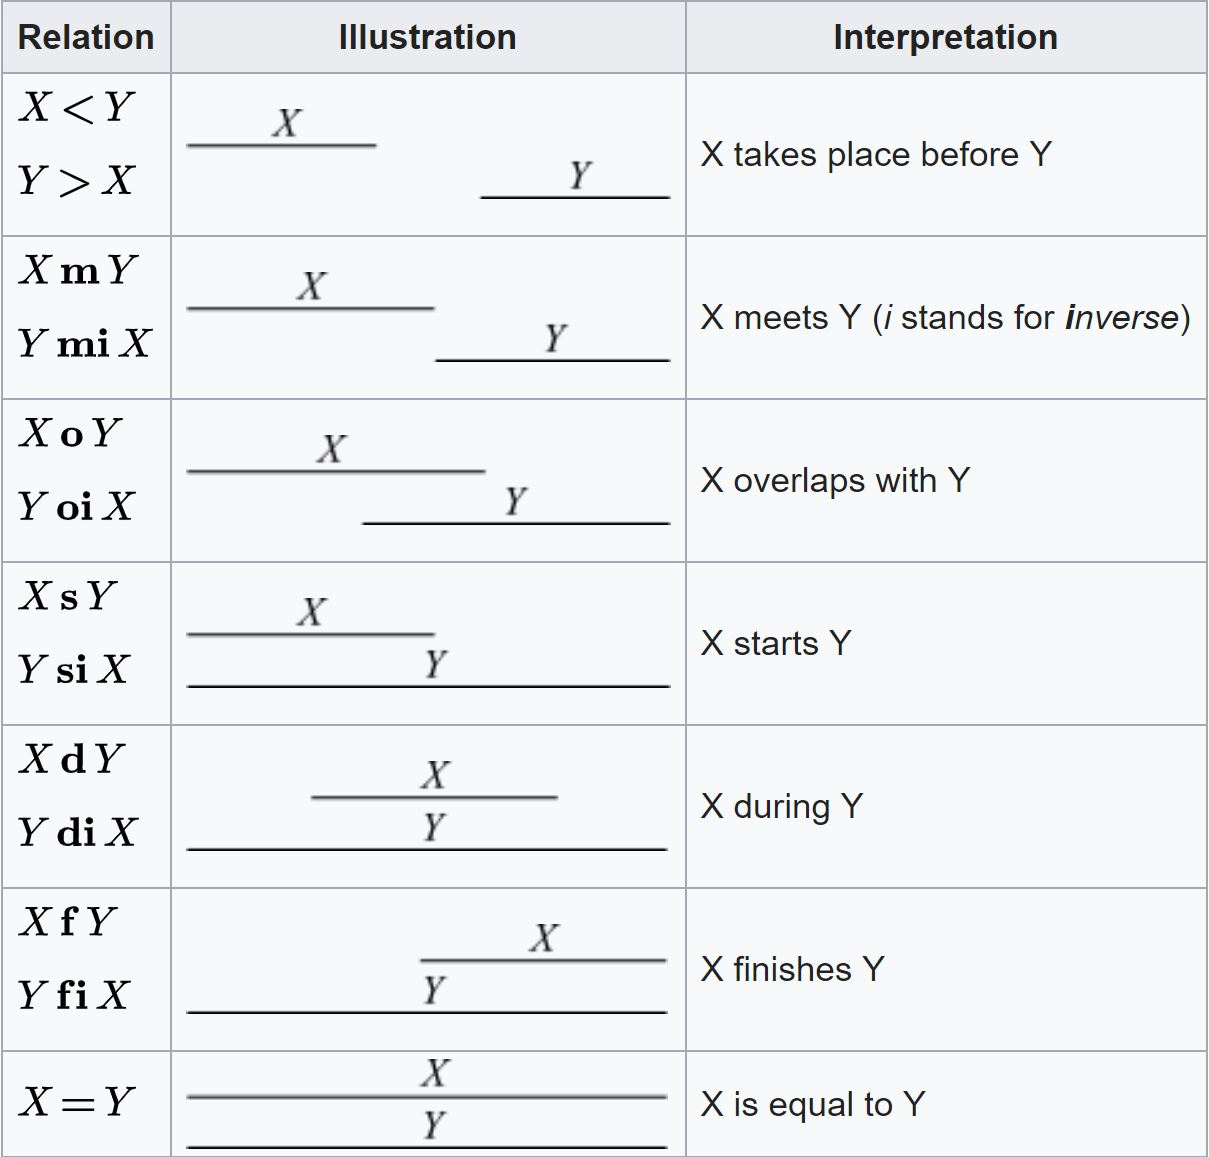
\includegraphics[scale=1]{allen}}
\end{figure}

Temporal information in languages can be conveyed in many ways. Verb tenses, specific temporal discourse markers or date, time, or duration expressions help identify necessary data. Background knowledge can also be a powerful determinant for detecting temporal information, but it is a harder method to convey into instructions that can be understood by a machine. Extraction systems work by directly associating time stamps. It is a straightforward and efficient method however it sacrifices recall, seeing how numerous events do not have associated timestamps.


\textbf{Conclusions}: Artificial intelligence and its sub-branches present powerful tools that can create applications that range from simple to intricate. They represent fields that are in continuous rapid development as more and more people are becoming interested in building machines capable of thinking on their own or executing human-specific tasks.
\newpage

\chapter{Conclusions}
Working with or learning temporal information can prove to be a daunting and overwhelming task at times. Many people usually resort to creating visual representations for this type of data in order to get an improved perspective and gain a better understanding. Creating visual depictions is not a recent activity and can be seen in many historical documents throughout time, but only in recent years, the possibility of using the digital environment in order to generate said imagery has become a more compelling idea.\par

The TimelineGenerator application was created with the purpose of offering a simple, free and easy-to-use service that can visually generate a timeline. Although its main target audience is students, it can be effortlessly used by anyone without requiring specific knowledge.\par

TimelineGenerator was created as a web application using a technology stack that includes elements ranging from well-known markup languages and standards such as HTML and CSS to libraries and APIs that are seldom seen and only used in specific contexts. The application uses a simple design to avoid unnecessary cluttering and gives the option to add events manually or with the help of a custom search engine which filters and processes Wikipedia articles. The latter feature is achieved with the help of specific APIs and JavaScript libraries and was added in order to facilitate the process of building a timeline. This characteristic has also been implemented on the basis of artificial intelligence and some of its representative braches such as natural language processing and temporal information extraction.\par

TimelineGenerator is not an intricate and complex web application with numerous features but it accomplishes its main goal by implementing straightforward services and keeping a clean look. Simple timelines can be effortlessly created by using this project and therefore users can obtain an essential visual representation of their acquired data.

\begin{figure}[h]
\vspace*{4cm}
\centerline{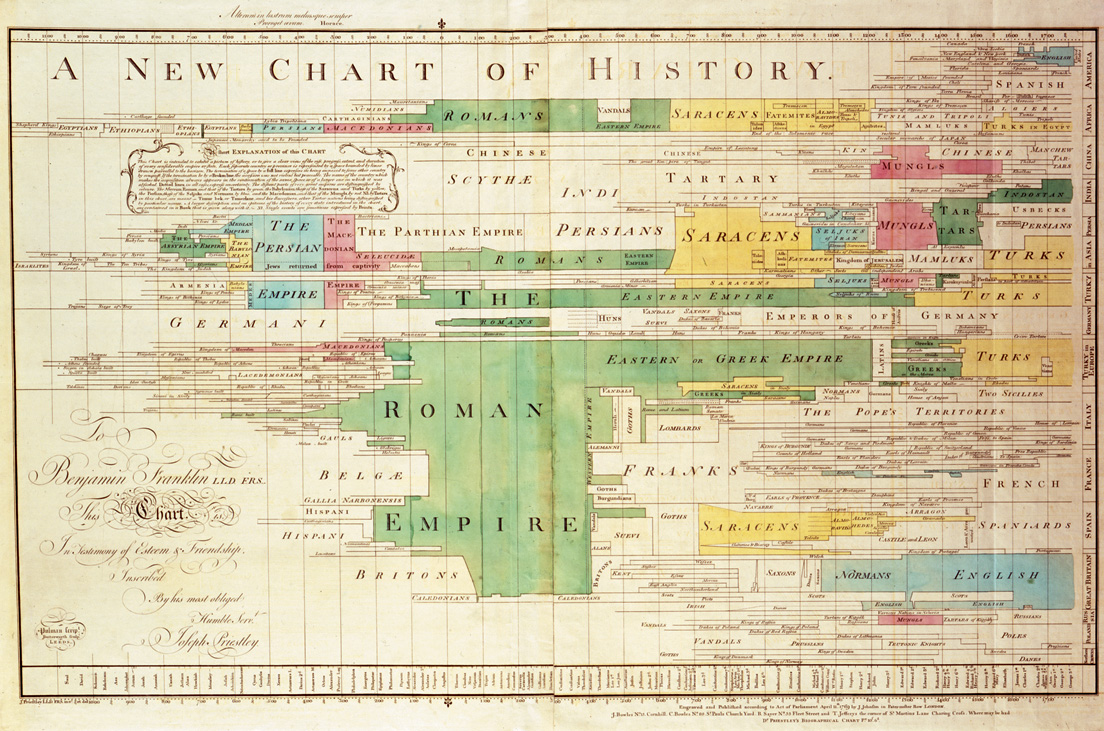
\includegraphics[scale=1.6]{htl}}
\caption{\textbf{Joseph Priestley}, 1765, A New Chart of History}
\end{figure}
\newpage

\section* {RESOURCES}
\begin{enumerate}
\item \textit{Harsimran Bedia Sangameshwar Patilb Swapnil Hingmireb Girish K. Palshikarb},  2017, \href{https://aclweb.org/anthology/W17-5912}{\textbf{Event Timeline Generation from History Textbooks}}, Department of CSE, IIT Patna, India, TCS Research, Pune, India;

\item \textit{Magic Web Solutions}, 2019 ,\href{https://www.magicwebsolutions.co.uk/blog/the-benefits-of-web-based-applications.htm}{\textbf{The benefits of web applications}};

\item \textit{Ethan Brown}, 2014, \href{http://www.vanmeegern.de/fileadmin/user_upload/PDF/Web_Development_with_Node_Express.pdf}{\textbf{Web development with Node \& Express}};

\item \textit{Tania Rascia}, 2015, \href{https://www.taniarascia.com/what-is-bootstrap-and-how-do-i-use-it/}{\textbf{What is Bootstrap}};

\item \textit{Kristian Kersting}, 2018, \href{https://ml-research.github.io/papers/kersting2018aiml_frontiers.pdf}{\textbf{Machine Learning and Artificial Intelligence: Two Fellow Travelers on the Quest for Intelligent Behavior in Machines}}, Machine Learning Lab, CS Department and Centre for Cognitive Science, Darmstadt University of Technology, Darmstadt, German;

\item \textit{Diksha Khurana, Aditya Koli, Kiran Khatter and Sukhdev Singh}, 2017, \href{https://arxiv.org/ftp/arxiv/papers/1708/1708.05148.pdf}{\textbf{Natural Language Processing: State of The Art, Current Trends and Challenges}}, Department of Computer Science and Engineering, Manav Rachna International University, Faridabad-121004, India, Accendere Knowledge Management Services Pvt. Ltd., India;

\item \textit{Elizabeth D. Liddy}, 2001, \href{https://surface.syr.edu/cgi/viewcontent.cgi?article=1043&context=istpub} {\textbf{Natural Language Processing}}, Syracuse University;

\item \textit{Michael J. Garbade}, 2018, \href{https://becominghuman.ai/a-simple-introduction-to-natural-language-processing-ea66a1747b32}{\textbf{A simple introduction to natural language processing}};

\item \textit{Nasir Safdari}, 2018, \href{https://towardsdatascience.com/named-entity-recognition-ner-meeting-industrys-requirement-by-applying-state-of-the-art-deep-698d2b3b4ede}{\textbf{Named Entity Recognition (NER) with keras and tensorflow}};

\item \textit{Archana Goyal, Manish Kumar, Vishal Gupta}, 2017,\href{https://pdfs.semanticscholar.org/2060/5fdae23f6e8d945deb22e09c46cecebb4f35.pdf}{\textbf{Named Entity Recognition: Applications, Approaches and Challenges}}, PG Department of Information Technology, GGDSD College (India), Department of Computer Science and Application, Panjab University Regional Centre, (India), University Institute of Engineering \& Technology,Panjab University (India);

\item \textit{Allen, J.F.}, 1981, \textbf{"An interval-based representation of temporal knowledge"}, Proc, 7th 1JCAI, Vancouver, B.C.;

\item \textit{Allen, J.F.}, 1984, \textbf{"Towards a General Theory of Action and Time"};

\item \textit{Artuur Leeuwenberg and Marie-Francine Moens}, 2018, \textbf{A Survey on Temporal Reasoning for Temporal Information Extraction from Text}, KU Leuven, Department of Computer Science, Celestijnenlaan 200A, 3001 Heverlee, Belgium;

\item \textit{Artuur Leeuwenberg and Marie-Francine Moens}, 2018, \href{https://aclweb.org/anthology/D18-1155}{\textbf{Temporal Information Extraction by Predicting Relative Time-lines}}, Department of Computer Science, KU Leuven, Belgium;

\item \textit{Xiao Ling and Daniel S. Weld}, 2010, \href{https://homes.cs.washington.edu/~weld/papers/ling-aaai10.pdf}{\textbf{Temporal Information Extraction}}, University of Washington, Department of Computer Science and Engineering, Seattle, WA 98195-2350, U.S.A.
\end{enumerate}
\end{document}